\section{Resultados e Discussão}
\label{sec:resultados}

Neste capítulo, são apresentados e discutidos os resultados obtidos a partir da implementação dos modelos propostos. A análise é dividida em duas grandes etapas: primeiramente, avalia-se o comportamento do sistema produtivo por meio da simulação computacional híbrida e sua respectiva visualização avançada, em seguida, apresenta-se a síntese do SED capaz de rastrear as falhas comportamentais observadas na simulação.

\subsection{Simulação Híbrida no AnyLogic}

A simulação híbrida, combinando a Modelagem Baseada em Agentes (ABM) e a Simulação a Eventos Discretos (DES), foi implementada no software AnyLogic. O protótipo computacional foi alimentado com os parâmetros e variáveis coletados empiricamente no canteiro de obras, incorporando os tempos de execução, as curvas de aprendizado, as percepções de dificuldade dos trabalhadores para cada atividade obrigatória da montagem e desmontagem das fôrmas e a disposição física da obra.

Primeiramente, foram estruturados os agentes da simulação: as fôrmas (\textit{Formworks}) e os trabalhadores (\textit{Workers}). No ambiente de modelagem AnyLogic, os agentes representam entidades com participação ativa ou passiva no sistema. Nesse sentido, as fôrmas atuam como os principais elementos de fluxo da DES, enquanto os trabalhadores representam os agentes autônomos da ABM.

\begin{figure}[!htb]
	\centering
	\caption{Propriedades do Agente fôrma.}
	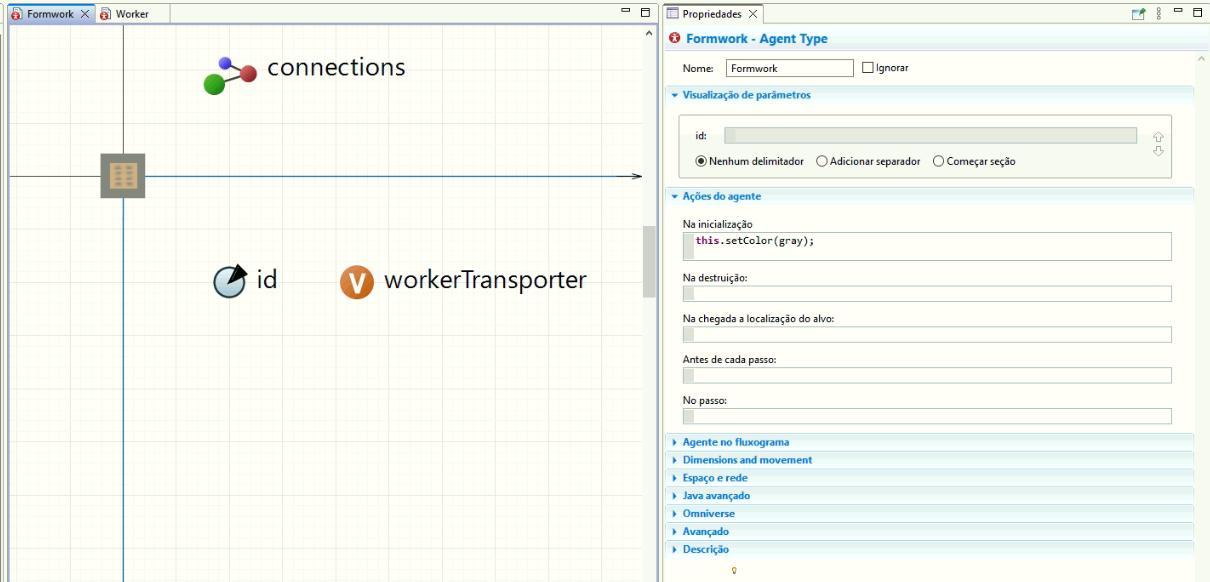
\includegraphics[width=0.8\textwidth]{Caps/Figs/formworks.jpeg}
	\fonte{Autoral.}
	\label{fig:formworks}
\end{figure}
\FloatBarrier

Conforme ilustrado na Figura \ref{fig:formworks}, cada fôrma possui um parâmetro de identificação exclusivo (\textit{id}) e armazena a informação do trabalhador associado responsável pelo seu transporte. No ambiente principal da simulação (\textit{Main}), o modelo foi projetado com arquitetura escalável para permitir a análise de múltiplas frentes de trabalho operando simultaneamente. Para isso, o Agente Fôrma foi instanciado em quatro populações distintas (Figura \ref{fig:formwork-population}). Cada população agrupa uma dupla de fôrmas direcionada a um setor específico da obra. Devido à sua natureza estática até serem manipuladas, a velocidade inicial desses agentes foi definida como zero, juntamente com a atribuição de sua localização espacial de origem. 

\begin{figure}[!htb]
	\centering
	\caption{Propriedades da população de fôrmas.}
	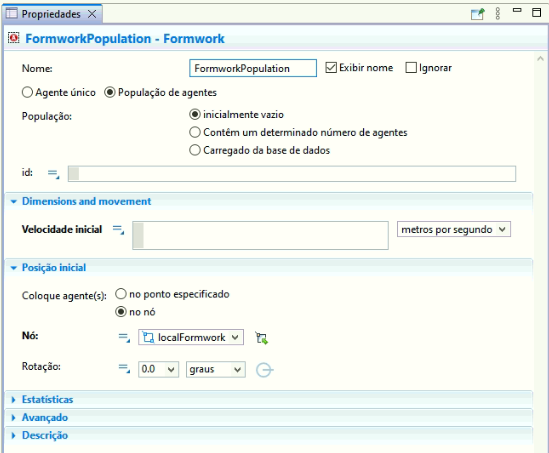
\includegraphics[width=0.6\textwidth]{Caps/Figs/formwork-population.png}
	\fonte{Autoral.}
	\label{fig:formwork-population}
\end{figure}
\FloatBarrier

De maneira análoga, foram criados os agentes dos trabalhadores e inseridos na \textit{Main} do projeto. Para espelhar a distribuição das fôrmas e manter a escalabilidade do canteiro, o Agente Trabalhador foi distribuído em quatro populações (Figuras \ref{fig:workers} e \ref{fig:workers-population}). Cada uma dessas populações é composta por uma dupla de operários, nascendo inicialmente vazias e sendo preenchidas dinamicamente durante a execução da simulação para atender aos respectivos setores.

\begin{figure}[!htb]
	\centering
	\caption{Propriedades do Agente trabalhador.}
	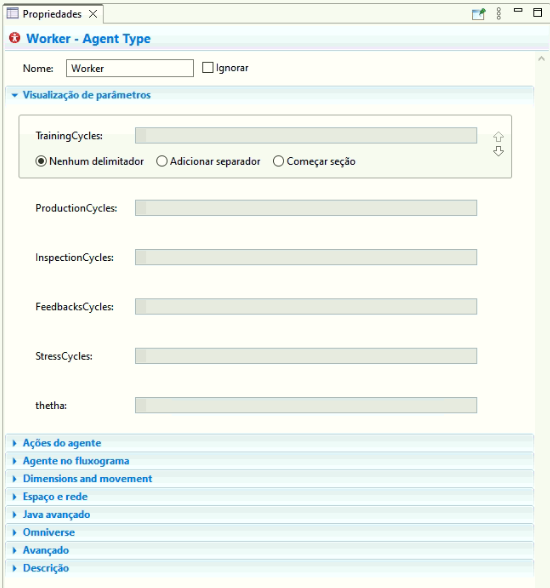
\includegraphics[width=0.6\textwidth]{Caps/Figs/workers.png}
	\fonte{Autoral.}
	\label{fig:workers}
\end{figure}
\FloatBarrier

\begin{figure}[!htb]
	\centering
	\caption{Propriedades da população de trabalhadores.}
	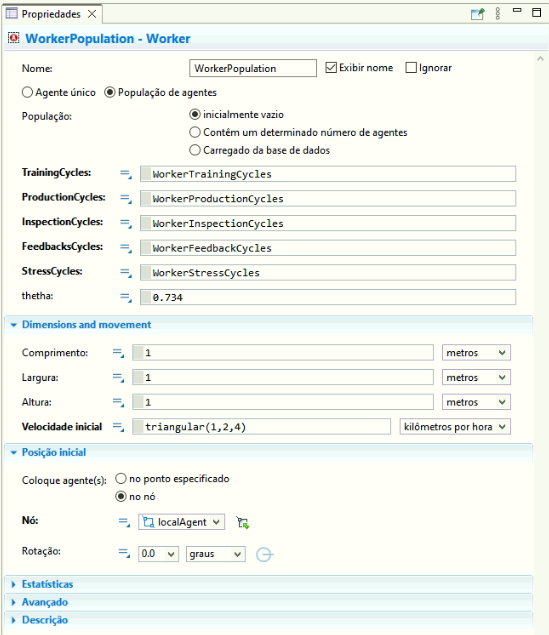
\includegraphics[width=0.6\textwidth]{Caps/Figs/workers-population.png}
	\fonte{Autoral.}
	\label{fig:workers-population}
\end{figure}
\FloatBarrier

Por serem os agentes centrais da arquitetura ABM, os trabalhadores carregam parâmetros individuais essenciais para o cálculo probabilístico do modelo cognitivo definido anteriormente na Equação \ref{eq:prob_cognitiva}. Tais parâmetros incluem os Ciclos de Treinamento (\textit{TrainingCycles}), Ciclos de Produção (\textit{ProductionCycles}), Ciclos de Inspeção (\textit{InspectionCycles}), Ciclos de Realimentação (\textit{FeedbackCycles}) e Ciclos de Estresse (\textit{StressCycles}). Os valores iniciais destas variáveis são carregados automaticamente a partir de um banco de dados externo em formato de planilha.

Diferentemente das fôrmas, os trabalhadores possuem mobilidade autônoma. A velocidade inicial de deslocamento desses agentes não é um valor constante, mas sim modelada por meio de uma distribuição probabilística triangular de parâmetros (1, 2, 4) representando a variabilidade da locomoção humana. Neste contexto, o valor 1 define a velocidade mínima, o valor 4 representa a velocidade máxima alcançável, e o valor 2 indica a moda, ou seja, a velocidade de caminhada mais provável e frequente durante a jornada de trabalho. Trabalhadores não têm um ID associado, haja visto que não é necessário identifica-los individualmente.

\subsubsection{DES no AnyLogic}

A abordagem DES foi responsável por definir a representação geométrica do espaço físico, delimitando as fronteiras de atuação dentro do ambiente \textit{Main} do AnyLogic. Para o dimensionamento e o posicionamento espacial dos elementos da simulação, foram utilizados os blocos construtivos \textit{Storage} e \textit{Rectangular Node}. Como mencionado previamente, a disposição espacial foi baseada nas obras do canteiro de obras A.

\begin{figure}[!htb]
	\centering
	\caption{Representação geométrica do cômodo e blocos no ambiente do AnyLogic.}
	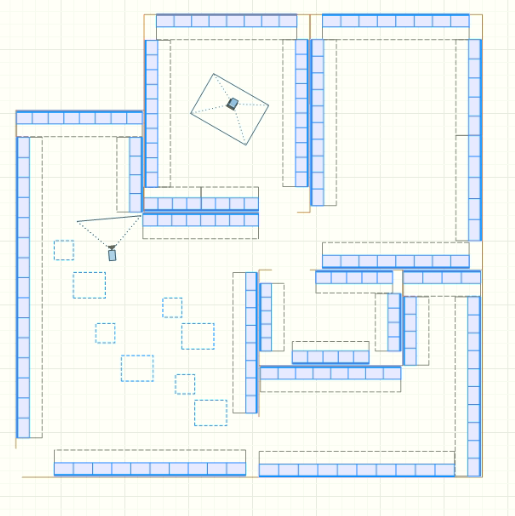
\includegraphics[width=0.8\textwidth]{Caps/Figs/des-vision.png} 
	\fonte{Autoral.}
	\label{fig:layout-des}
\end{figure}
\FloatBarrier

Para operacionalizar a movimentação física das fôrmas no ambiente simulado, utilizou-se o elemento \textit{Transporter Fleet} do Anylogic, configurado com o tipo de navegação de espaço livre. O \textit{Transporter Fleet} é um bloco capaz de definir e gerenciar um grupo de transportadores de outros agentes e  simular movimentações dentro do software, sendo utilizado para que os trabalhadores movam as fôrmas no canteiro. A capacidade dessa frota foi restrita a apenas dois agentes por cômodo, em estrita conformidade com as observações empíricas realizadas durante a coleta de dados no canteiro. Além de gerenciar a logística, o \textit{Transporter Fleet} atua como a principal ponte de comunicação entre a modelagem DES e a ABM. Conforme configurado na ação nativa \textit{On Release} (Figura \ref{fig:transporter}), assim que um trabalhador conclui a tarefa de montagem ou desmontagem de um painel, o sistema emite uma mensagem de "finalizado" (\textit{finished}). Essa mensagem é imediatamente capturada e processada pelo diagrama de estados (\textit{Statechart}) do agente trabalhador na ABM, que será visto mais a frente. Ao chegar ao destino final do transporte com "\textit{on destination reached}", ou seja, quando o trabalhador está montando as fôrmas é realizada uma transformação estética nas fôrmas para melhor visualização.

\begin{figure}[!htb]
	\centering
	\caption{Propriedades do \textit{Transporter Fleet} com movimentação livre.}
	 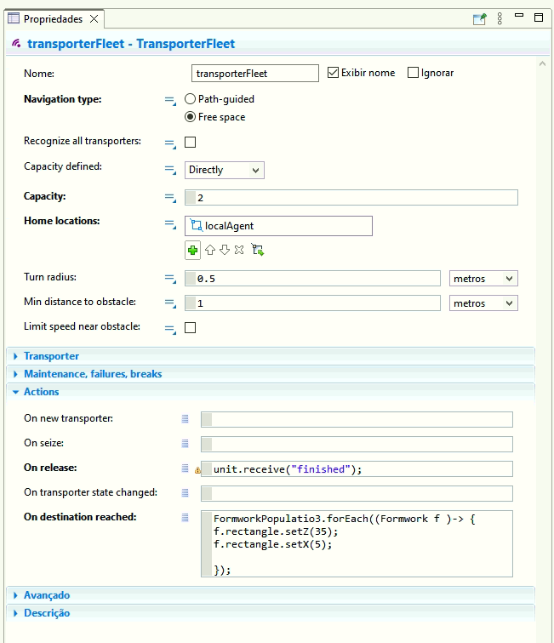
\includegraphics[width=0.8\textwidth]{Caps/Figs/transporter-fleet.png}
	\fonte{Autoral.}
	\label{fig:transporter}
\end{figure}
\FloatBarrier

A lógica de roteamento da montagem baseada em eventos discretos é estabelecida por uma cadeia de blocos interconectados (Figura \ref{fig:assembly-logic}). Após a inserção da fôrma no sistema pelo bloco \textit{Enter}, aplicou-se um bloco de \textit{Delay} de 1 segundo com o intuito de evitar sobrecarga computacional durante a simulação. Em seguida, o fluxo alcança o bloco \textit{SelectOutputln}, que atua como o controlador de roteamento. Esse bloco chama a função \textit{chooseOutput}, a qual é regida por condições lógicas que verificam continuamente a disponibilidade de espaço em cada parede. Uma vez que a capacidade máxima de uma parede é atingida, o fluxo é redirecionado para a próxima, até que a montagem de todo o ambiente seja concluída e as entidades saiam do sistema por meio do bloco \textit{Exit} (Figura \ref{fig:choose-output}).

\begin{figure}[!htb]
	\centering
	\caption{Conexão dos blocos na lógica de montagem.}
	 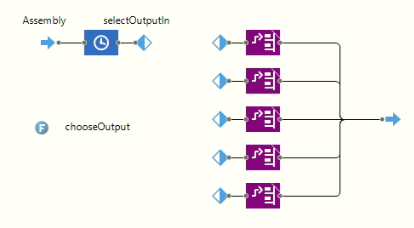
\includegraphics[width=0.5\textwidth]{Caps/Figs/assembly-logic.png}
	\fonte{Autoral.}
	\label{fig:assembly-logic}
\end{figure}
\FloatBarrier



\begin{figure}[!htb]
	\centering
	\caption{Propriedades lógicas da função \textit{chooseOutput}.}
	 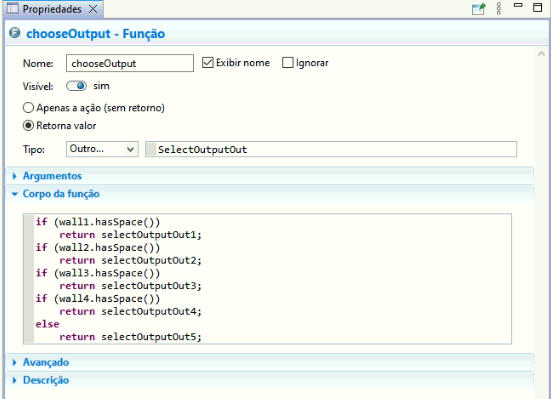
\includegraphics[width=0.8\textwidth]{Caps/Figs/chooseoutput.png}
	\fonte{Autoral.}
	\label{fig:choose-output}
\end{figure}
\FloatBarrier

Cada componente de montagem atrelado ao bloco \textit{Store} recebe configurações que definem o transportador utilizado, o local de busca da fôrma, o tempo de carregamento (baseado em uma distribuição triangular) e a liberação do trabalhador após a tarefa. O bloco \textit{Store} é utilizado para modelar o armazenamento de itens (agentes) em sistemas de armazenagem, como estantes, prateleiras ou racks. 

\begin{figure}[!htb]
	\centering
	\caption{Propiedades do bloco de armazenagem \textit{Store}.}
	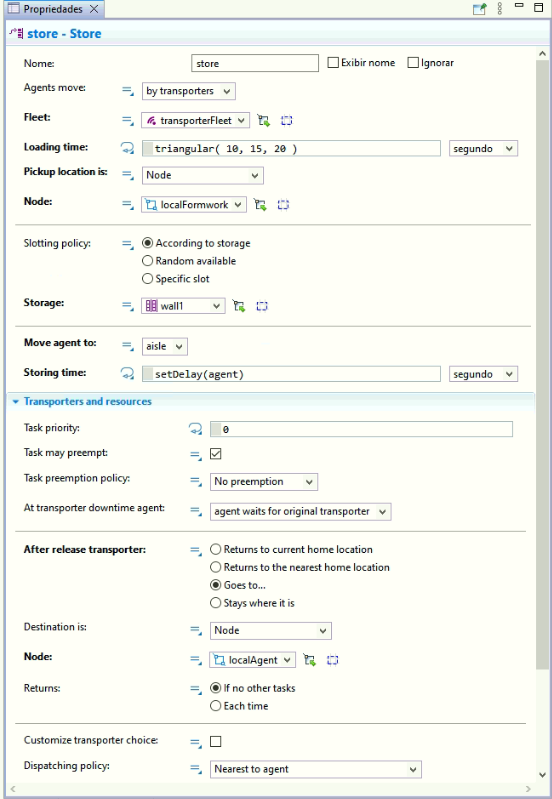
\includegraphics[width=0.6\textwidth]{Caps/Figs/store.png}
	\fonte{Autoral.}
	\label{fig:store}
\end{figure}
\FloatBarrier

O diferencial desta arquitetura híbrida reside na definição do tempo de armazenamento (equivalente ao tempo de montagem ou desmontagem da fôrma). Esse valor não é constante, ele é calculado dinamicamente por meio da função \textit{setDelay}, como mostra a Figura \ref{fig:setDelay}. Dentro da ABM, o trabalhador \textit{work} contém uma variável chamada \textit{CountDelay}. A cada etapa realizada pelo trabalhador, essa variável será incrementada com o tempo da etapa realizada. Se o trabalhador fizer pelo menos uma etapa, a flag de \textit{IsNeedDelay} é setada para \textit{True}. Dessa forma, \textit{CountDelay} acumula o tempo de realização das tarefas com base nas etapas executadas ou não executadas pelo trabalhador na ABM. Sendo assim, as decisões tomadas no nível cognitivo do agente refletem diretamente nos atrasos e no tempo físico computado pela DES.

\begin{figure}[!htb]
	\centering
	\caption{Função \textit{setDelay}.}
	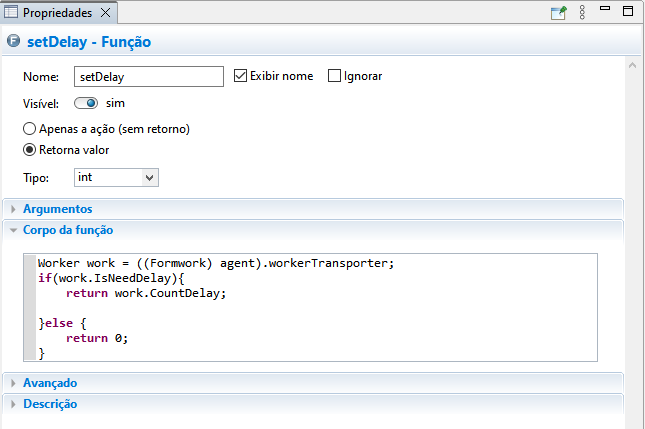
\includegraphics[width=0.8\textwidth]{Caps/Figs/setDelay.png}
	\fonte{Autoral.}
	\label{fig:setDelay}
\end{figure}
\FloatBarrier


A etapa de desmontagem foi feita de forma similar com a utilização do bloco \textit{Enter}, um bloco \textit{Delay} de 1 segundo e um bloco \textit{Retrieve}. O bloco \textit{Retrieve} é utilizado para remover agentes de um sistema de armazenagem. Destarte, o bloco \textit{Retrieve} realiza diretamente o processo de desmontagem. O bloco também usa a função \textit{setDelay} para retornar o tempo de desmontagem com base no tempo etapas de desmontagem realizadas ou não pelo trabalhador na ABM. Quando as fôrmas são removidas, o trabalhador as leva para a sua locação inicial, completando o ciclo da simulação.

\begin{figure}[!htb]
	\centering
	\caption{Conexão dos blocos na lógica de desmontagem.}
	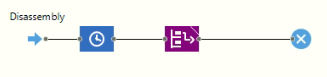
\includegraphics[width=0.5\textwidth]{Caps/Figs/disassembly-logic.png}
	\fonte{Autoral.}
	\label{fig:disassembly}
\end{figure}
\FloatBarrier

\begin{figure}[!htb]
	\centering
	\caption{Propiedades do bloco de desmonte \textit{Retrieve}.}
	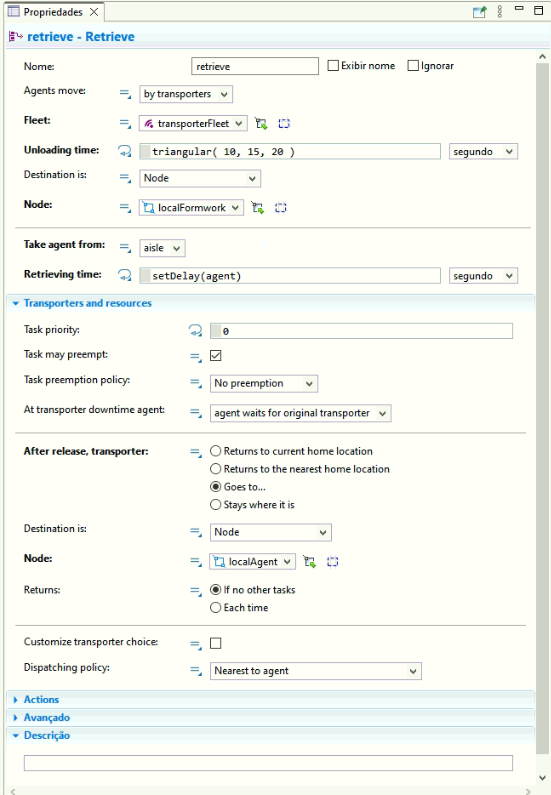
\includegraphics[width=0.5\textwidth]{Caps/Figs/retrieve.png}
	\fonte{Autoral.}
	\label{fig:retrieve}
\end{figure}
\FloatBarrier

Para concluir a etapa de DES, foram definidas duas \textit{flags} na função \textit{main}, responsáveis por controlar o estado da simulação: \textit{qAssembly} e \textit{qDissassembly}. Essas variáveis podem assumir valores binários (0 ou 1). Quando \textit{qAssembly} é igual a 0, a simulação encontra-se na etapa de montagem, a qual é considerada finalizada quando essa variável passa a valer 1.

\begin{figure}[!htb]
	\centering
	\caption{Variáveis para montagem e desmontagem.}
	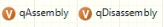
\includegraphics[width=0.3\textwidth]{Caps/Figs/qassembly.png}
	\fonte{Autoral.}
	\label{fig:qassembly}
\end{figure}
\FloatBarrier

Como as etapas são sequenciais, somente após a conclusão da montagem (\textit{qAssembly} = 1) é que se avalia o estado de \textit{qDissassembly}. Nesse caso, se \textit{qDissassembly} for igual a 0, a simulação está na etapa de desmontagem. Quando assume o valor 1, indica que ambas as etapas (montagem e desmontagem) foram concluídas.

\subsubsection{ABM no AnyLogic}
A abordagem ABM foi responsável por descrever o modelo cognitivo do trabalhador. A Figura \ref{fig:statechart} mostra o diagrama de estados do trabalhador, representado os estados possíveis do trabalhador no processo de montagem e desmontagem. O agente trabalhador inicia no modo Ocioso (\textit{Idle}). É no estado de Locomoção (\textit{Locomotion}) que está a lógica principal do trabalhador, seguido das etapas de montagem à esquerda e etapas de desmontagem à direita. Os útimos Estados definem se o comportamento do trabalhador foi adequado (\textit{AdeqBehaviorA}), concluindo todas as atividades, ou inadequado (\textit{InadeqBehavior}), pulando pelo menos uma atividade.

\begin{figure}[!htb]
	\centering
	\caption{Diagrama de estados na ABM.}
	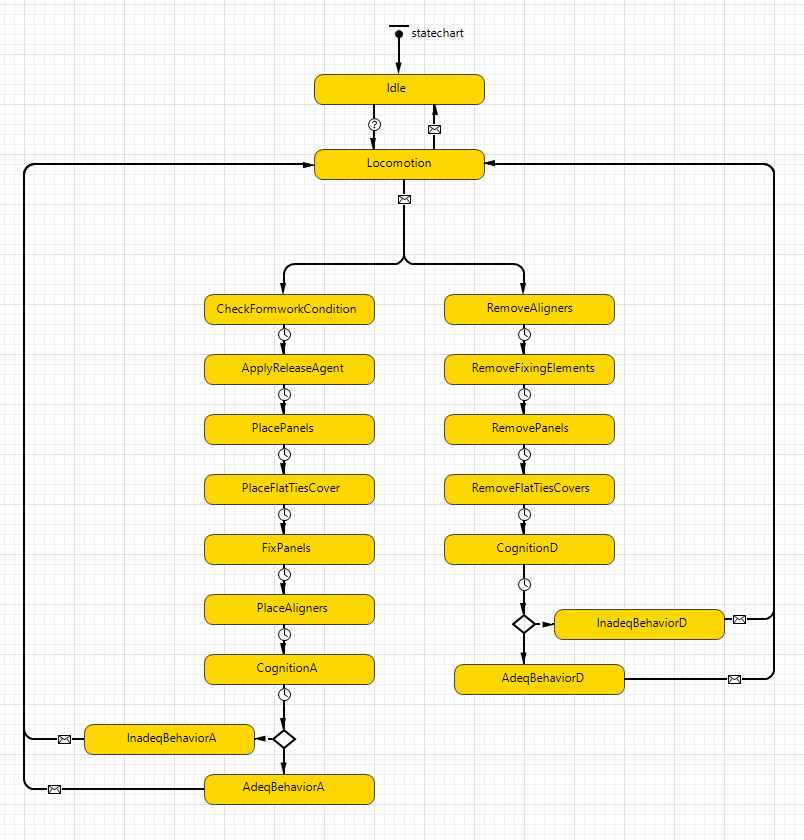
\includegraphics[width=0.8\textwidth]{Caps/Figs/stateChart.png}
	\fonte{Autoral.}
	\label{fig:statechart}
\end{figure}
\FloatBarrier

A transição para sair do estado Ocioso para o de Locomoção ocorre a partir de um Evento. No Anylogic, Eventos são elementos de modelagem utilizados para agendar e executar ações específicas em momentos definidos ou quando certas condições são atendidas no tempo de simulação.

\begin{figure}[!htb]
	\centering
	\caption{Eventos da ABM.}
	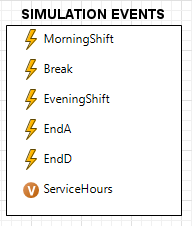
\includegraphics[width=0.3\textwidth]{Caps/Figs/Eventos.png}
	\fonte{Autoral.}
	\label{fig:eventos}
\end{figure}
\FloatBarrier

No contexto do projeto, o trabalhador sai do modo Ocioso quando as condições de tempo de trabalho são atendidas, ou seja, que foi iniciado o turno do serviço do trabalhador.

\begin{figure}[!htb]
	\centering
	\caption{Propriedades dos turnos.}
	
	\begin{minipage}{0.45\textwidth}
		\centering
		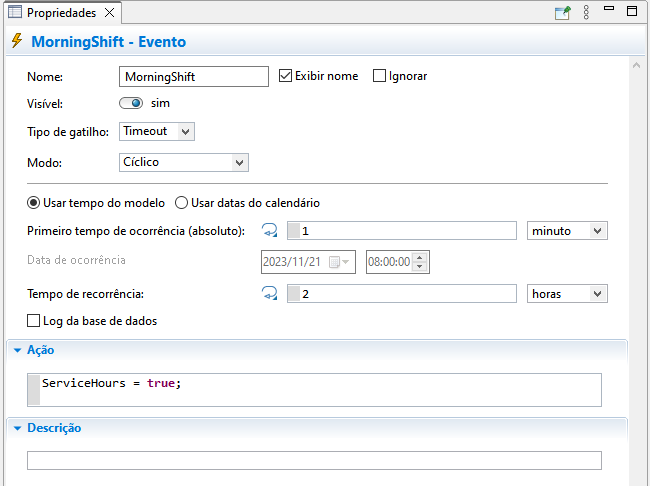
\includegraphics[width=\textwidth]{Caps/Figs/MorningShift.png}
		\caption*{(a) Morning Shift}
		\label{fig:morningShift}
	\end{minipage}
	\hfill
	\begin{minipage}{0.45\textwidth}
		\centering
		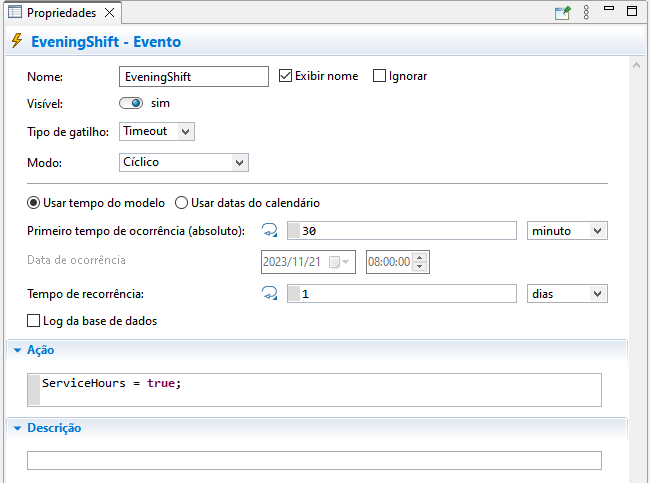
\includegraphics[width=\textwidth]{Caps/Figs/EveningShift.png}
		\caption*{(b) Evening Shift}
		\label{fig:eventos}
	\end{minipage}
	
	\fonte{Autoral.}
\end{figure}

\begin{figure}[!htb]
	\centering
	\caption{Propiedade do descanso \textit{Break}.}
	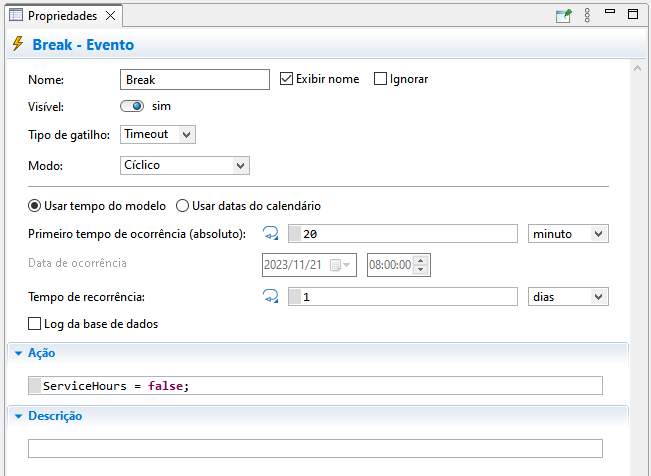
\includegraphics[width=0.45\textwidth]{Caps/Figs/Break.png}
	\fonte{Autoral.}
	\label{fig:eventos}
\end{figure}
\FloatBarrier



\subsection{ Visualização no NVIDIA Omniverse}
% Descrição: Apresente os resultados visuais e os insights que o 3D trouxe.
% O que abordar:
% - Imagens/prints do modelo renderizado no Omniverse.
% - Como a conexão dos dados do AnyLogic com o Omniverse facilitou a percepção espacial do canteiro.
% - Discussão sobre como ver os avatares (agentes) se movendo ajuda o gestor da obra a validar o modelo comportamental de forma muito mais intuitiva que apenas olhando gráficos 2D.

\subsection{Diagnóstico de Falhas por Sistemas a Eventos Discretos (SED)}
% Descrição: Faça uma ponte com a seção anterior. Diga que, como a simulação mostrou que as falhas ocorrem de forma velada, agora você aplicará o SED para detectá-las matematicamente.

\subsection{Autômato Gerador do Canteiro de Obras ($G$)}
% Descrição: É aqui que entra o grafo que desenha a tabela da metodologia.
% O que abordar:
% - Apresente a figura do grafo do autômato (as bolinhas de E0 a E11 e as setas das transições).
% - Discuta como as ramificações de falha (F1 a F5) criam caminhos paralelos que terminam no mesmo estado físico, ilustrando a "cegueira" do sistema de verificação tradicional.

\subsection{Síntese do Autômato Diagnosticador ($G_d$)}
% Descrição: Onde a mágica acontece. Você mostra o autômato observador que rastreia os eventos.
% O que abordar:
% - Apresente o grafo ou a tabela do Diagnosticador gerado.
% - Mostre como os estados agora carregam os rótulos (Normal, F1, F2, etc.).
% - Explique a evolução do diagnóstico: por exemplo, como o sistema percebe que a "Falha 3 (Omissão do desmoldante)" aconteceu logo após a leitura do evento observável O4.

\subsection{Análise de Diagnosticabilidade e Impactos na Gestão}
% Descrição: O fechamento de ouro juntando a engenharia com a matemática.
% O que abordar:
% - Confirme se o sistema é diagnosticável (se todas as falhas são descobertas antes que o ciclo da parede termine). Como o fluxo é finito (termina em E11), não deve haver ciclos indeterminados.
% - Discuta o impacto prático: como essa ferramenta matemática, integrada ao modelo de simulação, permitiria ao gestor da obra agir proativamente antes da concretagem, evitando o retrabalho pesado que você viu no AnyLogic.